\section{Algorithms}
\label{sec:algo}



\subsection{Distance to Nearest Wall}
\subsubsection{Feature Desciption}

\subsubsection{Mechanism}


sweep frequency chirp


Select Chirp Amplitude and Frequency

We firstly measure the ambient sound, and choose a quiet frequency.


What is chirp


why chirp?


How to generate chirp?


What chirp to use?


How to see echo? Time delay of echo, Shape of echo pulse, Phase Diff


SNR etc.

\fxnote{GRAPH: chirp and echo shape}


\subsection{Auto-correlation and Audio Reduction}

After receiving the original sound and echo, we do auto-correlation with original sound,
and remove it from the audio track.

\fxnote{GRAPH: how auto-correlation works}


\subsubsection{Determine Envelops}

Envelop is the sound of big surface. Physical expalination. 
Define envelop as the same duration of original sound.

\begin{figure}[H]
\centering
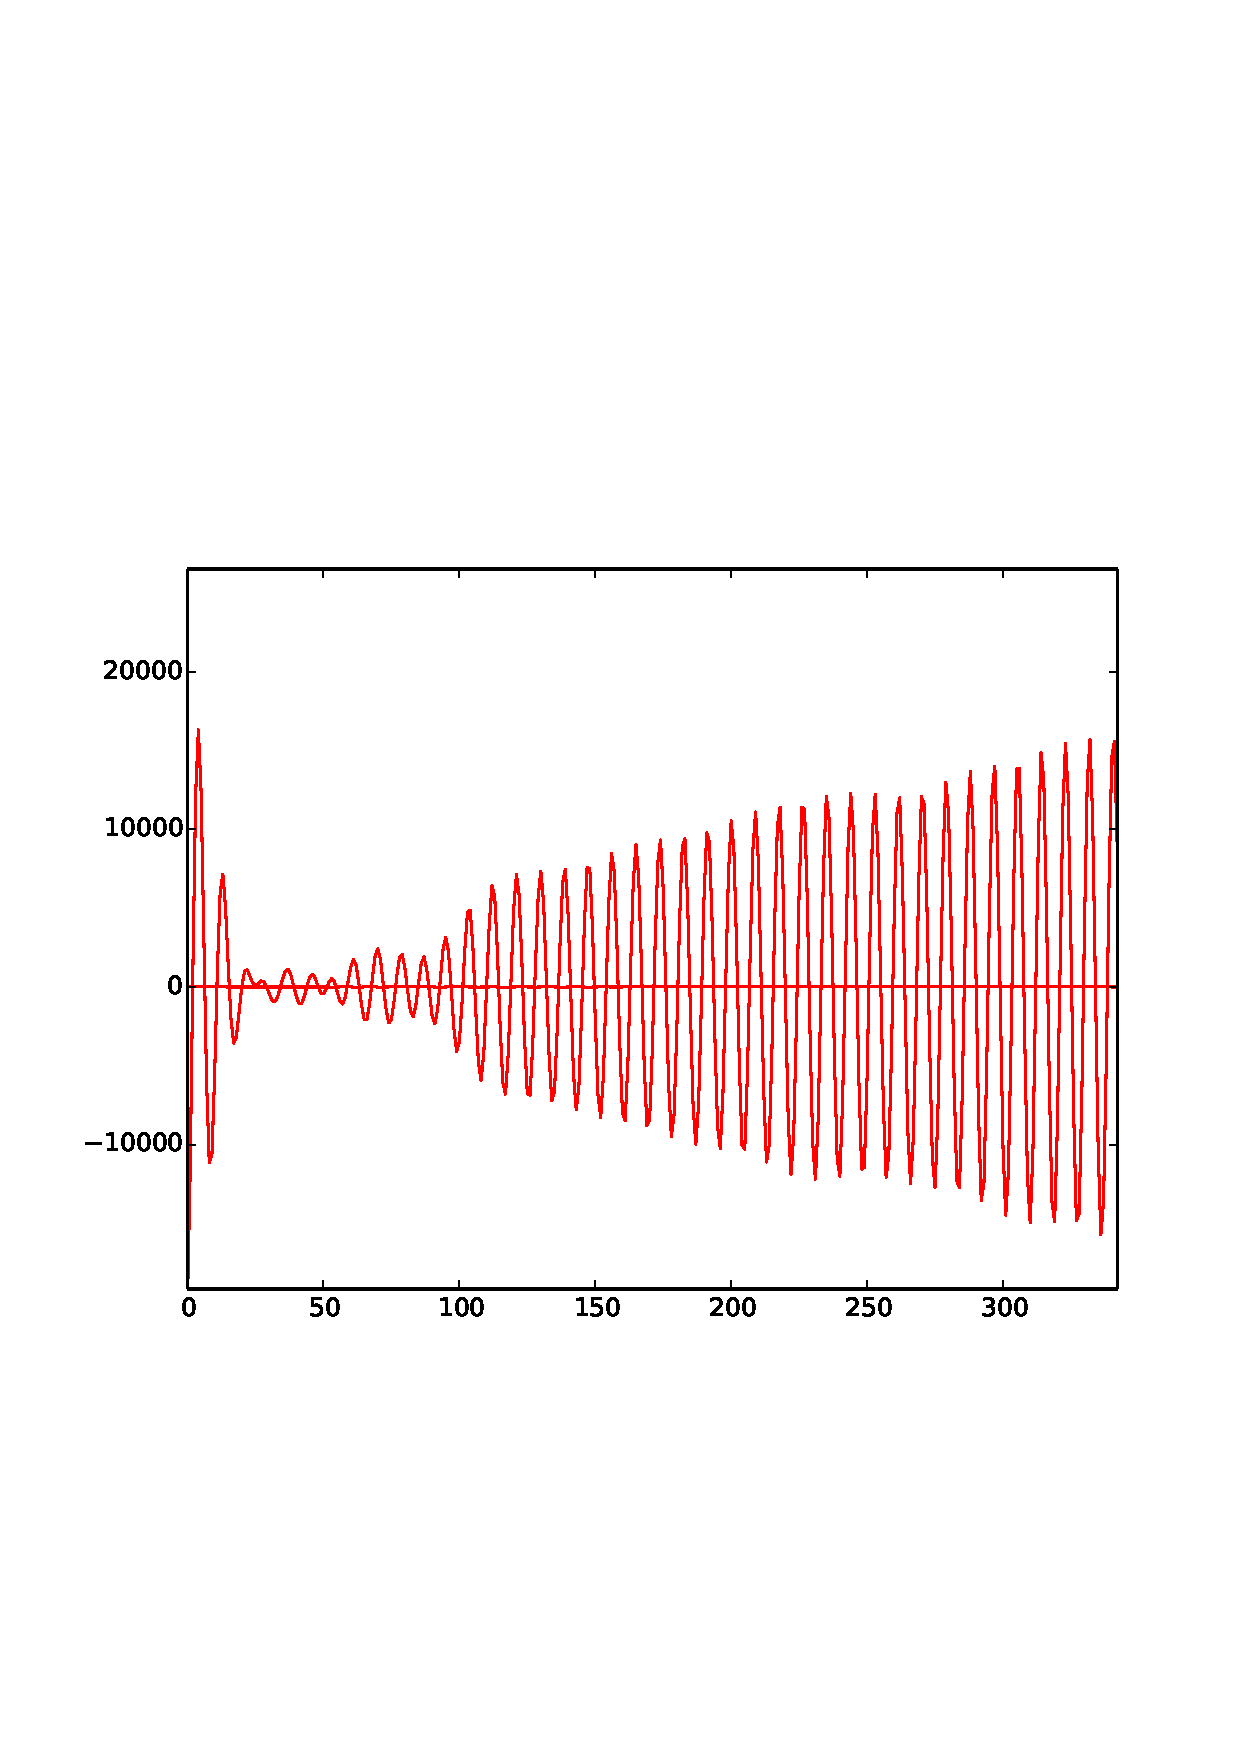
\includegraphics[width=0.45\textwidth]{./fig/40cm.pdf}
\caption{System Architecture of Drummer}
\end{figure}

\begin{figure}[H]
\centering
\includegraphics[width=0.45\textwidth]{./fig/inroom.pdf}
\caption{System Architecture of Drummer}
\end{figure}



\subsubsection{Phase Diff}



\subsubsection{Shape of Echo}


\fxnote{GRAPH: envelop shapes}

\subsubsection{Iterative Audio Reduction}

We remove the acoustic effects of an object after determining its existence, and 
in turn investigate the remaining sound iteratively. 


\subsubsection{Determine Direction of Each Object}

We use accelerometer to measure movements, and redo probing several time, and 
use TDoA of envelops to determine the direction of the object represented by the envelop.


Binaural beat


\subsection{Sudden Change of Enclosing Physical Environment}

\subsubsection{Feature Desciption}

\subsubsection{Mechanism}
